\chapter{Customer Site Usage}

Using the site as a non-administrative user allows the user to add seats to the user's shopping cart, make seating reservations, and change their own login information (such as address information and password).

\section{Creating a User}

To use the site as a non-administrative user, a customer needs to create a user on the site. This is accomplished by going to the login page and clicking on the ``signup'' link.

\begin{figure}[ht]
    \centering
    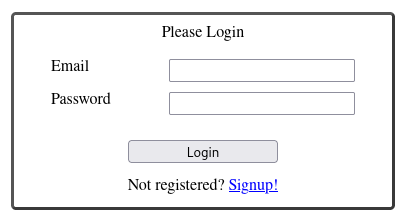
\includegraphics[width=8cm]{images/chapter3/login form}
    \caption{Login Form With Signup Link}
    \label{ref:login_form}
\end{figure}

Clicking on the signup link prompts the user for an email address, first name, last name, address information, and a password. Once the required info has been submitted, the server will verify that the email address is unique. Provied the email address IS unique and the password matches the password confirmation, the user will be created on the site.

Alternatively, a user may be created by an administrative user as shown in \hyperref[sec:managing_users]{\textcolor{blue}{\underline{Managing Users}}}. A list of all users on the site may be viewed there as well.

Once the user has been created, the user may login at any time by visiting the login page. After login, the user will be able to \hyperref[sec:reserving_seats]{\textcolor{blue}{\underline{Reserve Seats}}} and \hyperref[sec:modifying_account_information]{\textcolor{blue}{\underline{modify their account information}}}.

\section{Reserving Seats}\label{sec:reserving_seats}

After a user has logged in, the user may add seats to their shopping cart and reserve the seats. To prevent a user from locking out all seats by selecting all seats and then never completing a reservation, the seats in the shopping cart are not locked out until a reservation is made. Once a reservation is made, the seats become unavailable to any other users.

To add carts, to the shopping cart, the user must select a play from the Plays screen.

\begin{figure}[ht]
    \centering
    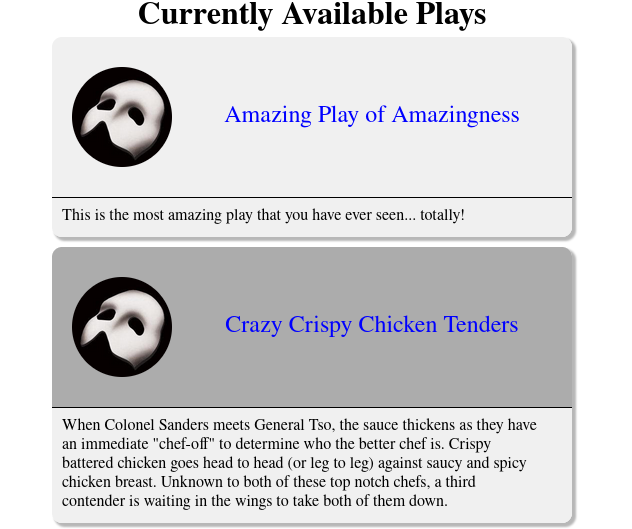
\includegraphics[width=8cm]{images/chapter3/play selection}
    \caption{Selecting a Play}
    \label{fig:play_selection}
\end{figure}

After selecting a play, the user will be shown a screen with the seating for this play. Blue seats are available, grey seats are reserved, and orange seats are currently in the shopping cart. As can be seen in figure \ref{fig:play_seating_selection}, three seats are unavailable (already reserved), four seats are in the shopping cart, and the remaining seats are available for reservation.

\begin{figure}[ht]
    \centering
    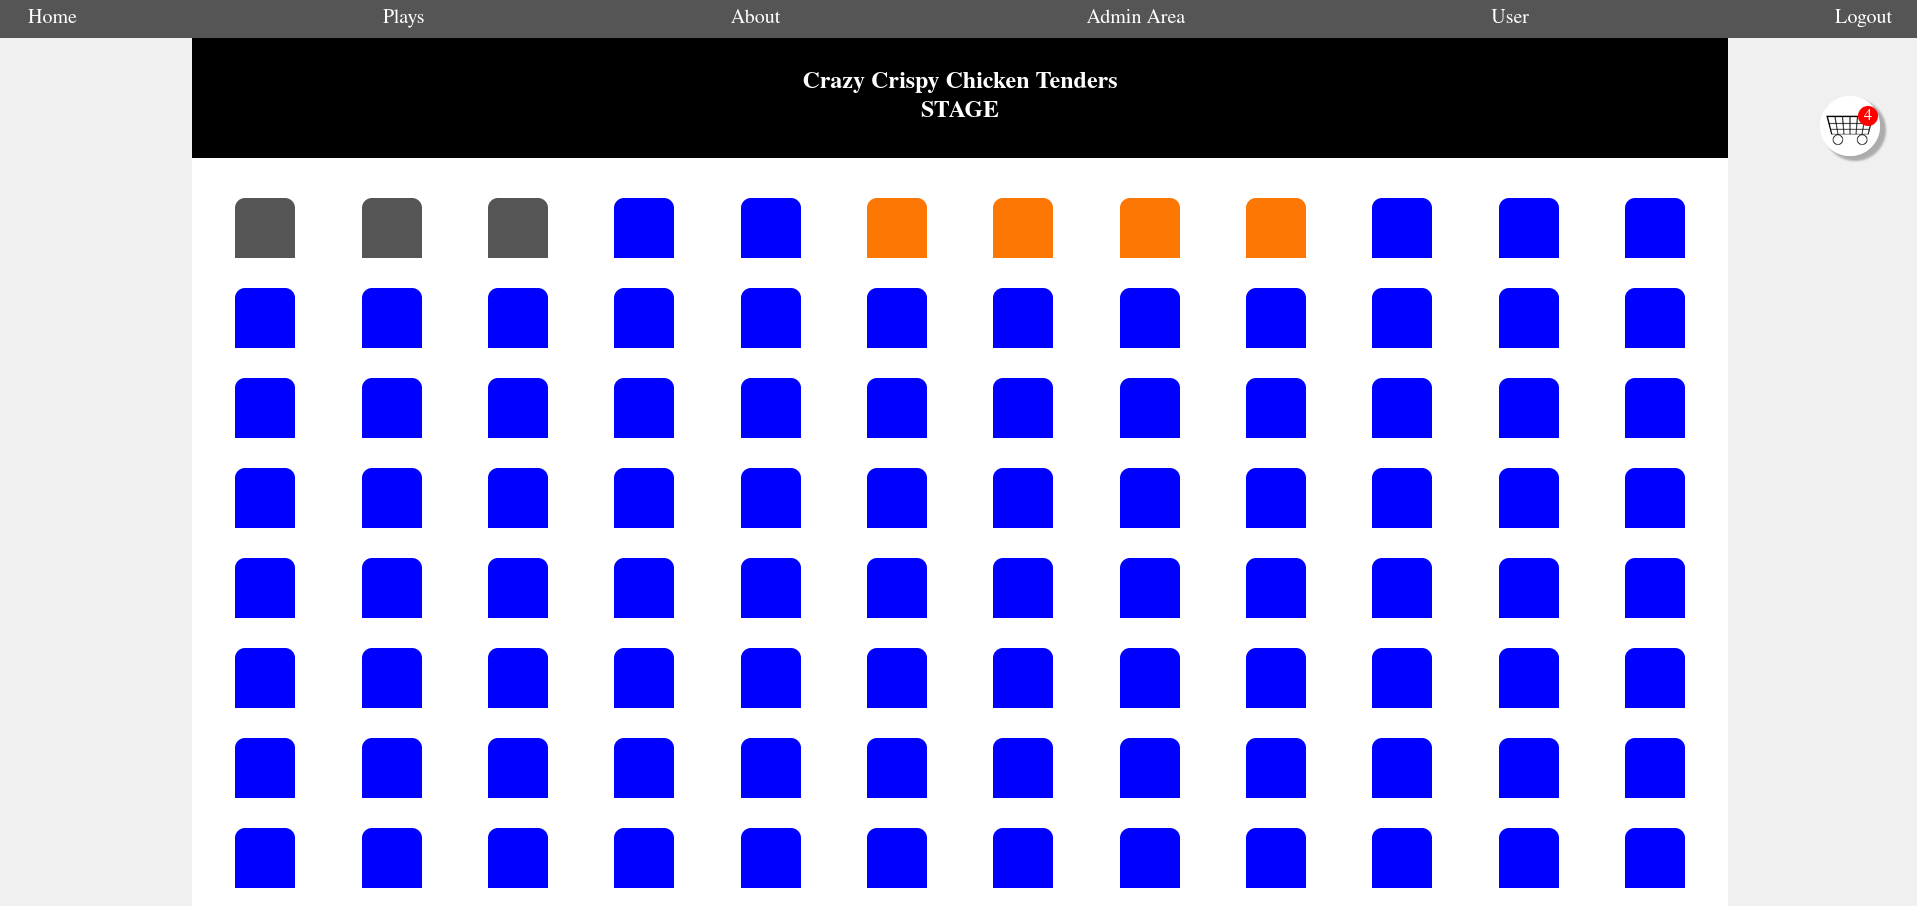
\includegraphics[width=10cm]{images/chapter3/play seating selection}
    \caption{Selecting Seats}
    \label{fig:play_seating_selection}
\end{figure}

After selecting seats, the user may click on the floating shopping cart icon in the top right side of screen. This allows the user to view their shopping cart.

\begin{figure}[ht]
    \centering
    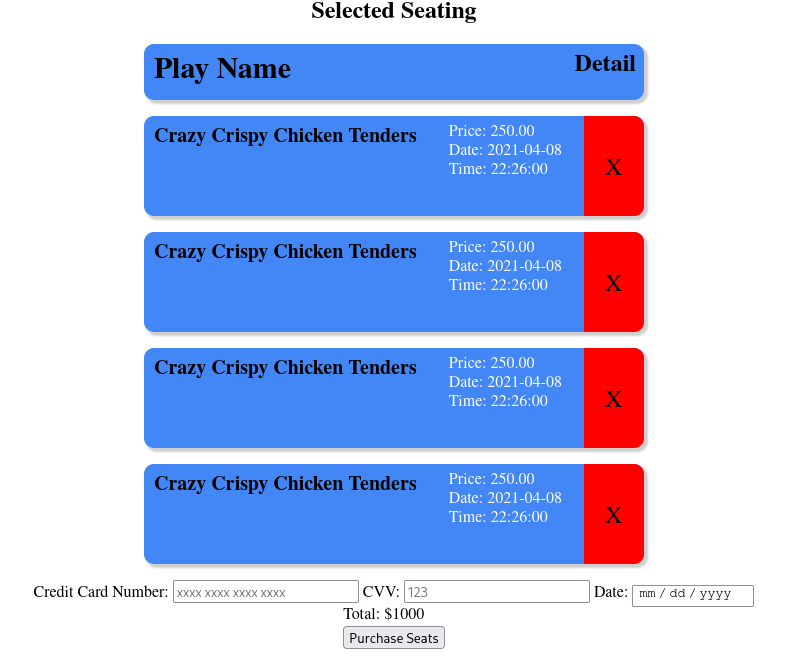
\includegraphics[width=8cm]{images/chapter3/shopping cart contents}
    \caption{Contents of the Shopping Cart}
    \label{fig:shopping_cart_contents}
\end{figure}

The user may remove items from their shopping cart at this point if they so desire. This is accomplished by clicking on the red tab with an "x" in it. When hovering over this tab, the tab becomes orange to indicate that changes will happen if clicked.

\begin{figure}[ht]
    \centering
    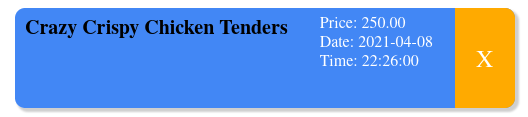
\includegraphics[width=8cm]{images/chapter3/shopping cart item removal}
    \caption{Removing a Shopping Cart Item}
    \label{fig:shopping_cart_item_removal}
\end{figure}

Once the item has been removed, the screen will be updatd with the current items in the cart. As would be expected, the current items will no longer include the item that has been removed.

\begin{figure}[ht]
    \centering
    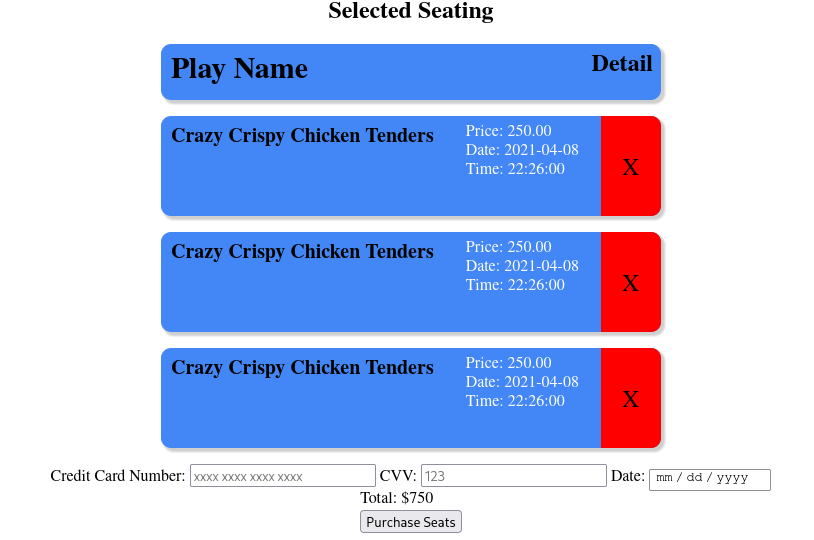
\includegraphics[width=8cm]{images/chapter3/shopping cart after removal}
    \caption{Shopping Cart After Removal}
    \label{fig:shopping_cart_after_removal}
\end{figure}

Once the user is ready to proceed with their purchase, they must enter their credit card information in the provided section (credit card, CV, and expiration date). After entering this information, they simply click on ``Purchase Seats'' to reserve those seats.

After the seats are reserved, the user will be shown a report containing the seats reserved. This report includes the play name, the date and time of the play, the total amount of the purchsed items, and the row/seat that has been reserved.

\begin{figure}[ht]
    \centering
    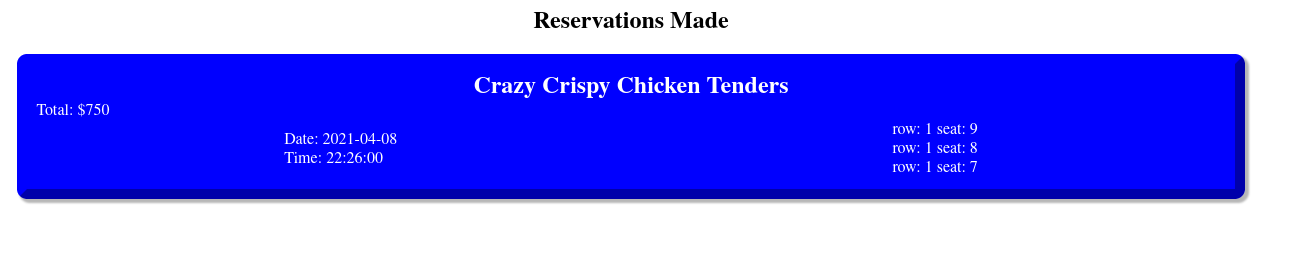
\includegraphics[width=8cm]{images/chapter3/reservations made}
    \caption{Reservations Made}
    \label{fig:reservations_made}
\end{figure}

\clearpage

\section{Modifing Account Information}\label{sec:modifying_account_information}

Users are allowed to modify their own account information at any time. This is accomplished by clicking on the user link at the top of the page while logged in.

\begin{figure}[ht]
    \centering
    
\includegraphics[width=8cm]{images/chapter3/user link}
    \caption{User Link}
    \label{fig:user_link}
\end{figure}

Once clicked, the edit user form will be opened.

\begin{figure}[ht]
    \centering
    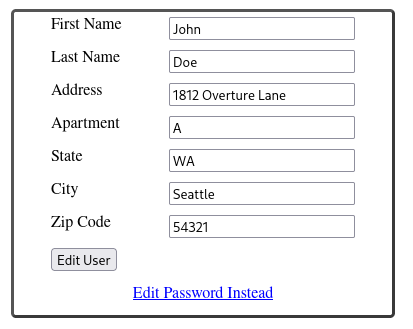
\includegraphics[width=8cm]{images/chapter3/edit user form}
    \caption{Edit User Form}
    \label{fig:edit_user_form}
\end{figure}

The edit user form allows the user to modify their first name, last name, and address information. If the user instead wishes to modify their password, they may click on ``Edit Password Instead'' link at the bottom of the form.

Clicking ``Edit User'' will save any changes that were made. If no changes were made, the user will remain as it was.
